% SC2207 --- Chapter 3: SQL (0->100)
\chapter{SQL: Definition, Manipulation, and Querying}
\label{ch:sql}

\begin{quote}
\emph{``SQL is the lingua franca of data.''} Algebra is elegant on paper; SQL is how tables are actually created, filled, and queried in every DBMS from SQLite to BigQuery.
\end{quote}

\noindent\fbox{\parbox{\dimexpr\linewidth-2\fboxsep-2\fboxrule}{%
\textbf{From zero: algebra $\to$ SQL.} We assume only the relational model of Ch.~2 (tables, keys, $\sigma$/$\pi$/$\bowtie$). No prior SQL is assumed; every clause is introduced with an algebra gloss and a runnable example.}}
\vspace{0.4em}

\section*{Learning Outcomes}
After this chapter you will be able to:
\begin{enumerate}[label=(L\arabic*)]
    \item write DDL to create, alter, and drop tables with keys and checks;
    \item write DML to insert, update, and delete rows correctly;
    \item compose SELECT with WHERE, JOIN, GROUP BY, HAVING, ORDER BY, and subqueries;
    \item define and use views and explain updatability limits;
    \item translate between relational algebra and SQL and predict bag vs.\ set behaviour.
\end{enumerate}

% ============================================================
\section{DDL: Creating the Schema}
\label{sec:ddl}

Data Definition Language declares the schema; the DBMS enforces it henceforth. Think ``define the blueprint before laying bricks.''

\begin{lstlisting}[language=SQL, caption={DDL for NTU mini-schema}, label={lst:ddl}]
CREATE TABLE Student(
  id      CHAR(9) PRIMARY KEY,
  name    VARCHAR(64) NOT NULL,
  major   VARCHAR(32) DEFAULT 'CS',
  gpa     DECIMAL(3,2) CHECK (gpa BETWEEN 0.00 AND 5.00)
);
CREATE TABLE Course(
  code    CHAR(6) PRIMARY KEY,
  title   VARCHAR(64) NOT NULL,
  credits INT CHECK (credits IN (3,4))
);
CREATE TABLE Enrolled(
  studID  CHAR(9) REFERENCES Student(id) ON DELETE CASCADE,
  code    CHAR(6) REFERENCES Course(code) ON DELETE CASCADE,
  grade   INT CHECK (grade BETWEEN 0 AND 100),
  PRIMARY KEY (studID, code)
);
\end{lstlisting}

Key DDL elements: types (\texttt{CHAR}, \texttt{VARCHAR}, \texttt{INT}, \texttt{DECIMAL}, \texttt{DATE}), \texttt{NOT NULL}, \texttt{DEFAULT}, \texttt{CHECK}, \texttt{PRIMARY KEY}, \texttt{FOREIGN KEY \ldots REFERENCES}, \texttt{UNIQUE}. Actions on FK violation: \texttt{CASCADE} (propagate), \texttt{SET NULL}, \texttt{RESTRICT/NO ACTION} (reject), \texttt{SET DEFAULT}. \texttt{ALTER TABLE} adds/drops columns or constraints; \texttt{DROP TABLE} (with \texttt{CASCADE}) removes it.

\begin{remark}[Domains in SQL]
SQL domains are coarser than pure relational domains: \texttt{CREATE DOMAIN GPA AS DECIMAL(3,2) CHECK(\ldots)} can reuse a constrained type across tables.
\end{remark}

% ============================================================
\section{DML: Inserting, Updating, Deleting}
\label{sec:dml}

Data Manipulation Language changes instances. Each statement is a transaction step (committed in Ch.~7).

\begin{lstlisting}[language=SQL, caption={DML examples}, label={lst:dml}]
INSERT INTO Student VALUES ('U1234567A','Ann Tan','CS',4.52);
INSERT INTO Enrolled(studID, code) VALUES ('U1234567A','SC2207'); -- grade NULL

UPDATE Student SET gpa = 4.65 WHERE id='U1234567A';
UPDATE Enrolled SET grade = 88
 WHERE studID='U1234567A' AND code='SC2207';

DELETE FROM Enrolled WHERE grade < 50;   -- withdraw fails
DELETE FROM Student WHERE id='U1234567A'; -- cascades to Enrolled
\end{lstlisting}

Constraints checked per row; the statement rolls back on violation. Bulk insert: \texttt{INSERT INTO \ldots SELECT \ldots}. Upsert (PostgreSQL/MySQL): \texttt{ON CONFLICT \ldots DO UPDATE}. Beware bag semantics: inserting a duplicate PK fails, but inserting duplicate non-key rows succeeds (unlike set algebra).

% ============================================================
\section{SELECT: The Query Workhorse}
\label{sec:select}

Every SELECT maps to algebra: \texttt{FROM} ($\times$/$\bowtie$) $\to$ \texttt{WHERE} ($\sigma$) $\to$ \texttt{GROUP BY} + aggregation $\to$ \texttt{HAVING} ($\sigma$ on groups) $\to$ \texttt{SELECT} ($\pi$) $\to$ \texttt{ORDER BY} $\to$ \texttt{LIMIT}.

\begin{figure}[h]
\centering
\begin{tikzpicture}[scale=0.74, every node/.style={font=\scriptsize},
  b/.style={draw, thick, rounded corners, align=center, minimum width=2.0cm, minimum height=0.6cm}]
  \node[b, fill=blue!13] (fr) at (0,3.0) {FROM / JOIN\\{\tiny $\times$, $\bowtie$}};
  \node[b, fill=green!13] (wh) at (0,2.2) {WHERE\\{\tiny $\sigma$}};
  \node[b, fill=orange!15] (gb) at (0,1.4) {GROUP BY\\{\tiny partition}};
  \node[b, fill=violet!12] (hv) at (0,0.6) {HAVING\\{\tiny $\sigma$ on groups}};
  \node[b, fill=red!12] (se) at (0,-0.2) {SELECT\\{\tiny $\pi$ (+ exprs)}};
  \node[b, fill=teal!12] (ob) at (0,-1.0) {ORDER BY + LIMIT};
  \foreach \a/\b in {fr/wh, wh/gb, gb/hv, hv/se, se/ob} \draw[-{Stealth}, thick, blue!60!black] (\a)--(\b);
  \node[font=\tiny, fill=yellow!10, draw, rounded corners, inner sep=2pt, align=left] at (4.5,1.4) {Logical order $\neq$\\written order:\\FROM first,\\SELECT near-last.};
\end{tikzpicture}
\caption{Logical evaluation order of SELECT. Optimisers reorder but preserve this semantics.}
\label{fig:select-order}
\end{figure}

\subsection{Filtering and Projection}

\begin{lstlisting}[language=SQL, caption={WHERE and SELECT}, label={lst:where}]
-- Algebra: pi_Name(sigma_major='CS'(Student))
SELECT DISTINCT name FROM Student WHERE major='CS';

-- Pattern, range, null
SELECT * FROM Student WHERE name LIKE 'Tan %' AND gpa BETWEEN 3.5 AND 5.0;
SELECT * FROM Enrolled WHERE grade IS NOT NULL;
\end{lstlisting}

\texttt{DISTINCT} de-duplicates to match set semantics; default \texttt{ALL} keeps bags (faster). \texttt{LIKE} with \texttt{\%} (any) and \texttt{\_} (one char); \texttt{BETWEEN}, \texttt{IN}, \texttt{IS NULL} test null correctly (\texttt{= NULL} is always unknown).

\subsection{JOINs}

\begin{lstlisting}[language=SQL, caption={JOIN variants}, label={lst:join}]
-- Inner (natural on studID) vs explicit condition
SELECT S.name, E.grade
  FROM Student S JOIN Enrolled E ON S.id = E.studID
 WHERE E.code='SC2207';

-- Left outer: every student, even with no enrolment
SELECT S.name, E.code FROM Student S LEFT JOIN Enrolled E ON S.id=E.studID;

-- Self-join: pairs of students in same course
SELECT A.studID, B.studID
  FROM Enrolled A JOIN Enrolled B
    ON A.code=B.code AND A.studID < B.studID;
\end{lstlisting}

Types: \texttt{[INNER] JOIN}, \texttt{LEFT/RIGHT/FULL OUTER JOIN}, \texttt{CROSS JOIN} ($\times$), \texttt{NATURAL JOIN}. Outer joins pad with \texttt{NULL}. Join order matters for outer joins but not inner (optimizer picks cheapest).

\begin{figure}[h]
\centering
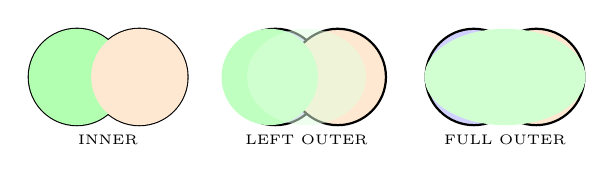
\begin{tikzpicture}[scale=0.72, every node/.style={font=\tiny}]
  \begin{scope}
    \draw[thick, fill=blue!18] (0,0) circle (0.85);
    \draw[thick, fill=orange!18] (1.1,0) circle (0.85);
    \node at (-0.35,0.3) {S}; \node at (1.45,0.3) {E};
    \fill[green!30] (0,0) circle (0.85); \fill[orange!18] (1.1,0) circle (0.85);
    \node at (0.55,-1.1) {INNER};
  \end{scope}
  \begin{scope}[xshift=3.5cm]
    \draw[thick, fill=blue!18] (0,0) circle (0.85);
    \draw[thick, fill=orange!18] (1.1,0) circle (0.85);
    \fill[green!25] (-0.1,0) circle (0.85); \fill[green!12, opacity=0.5] (0.55,0) ellipse (1.05 and 0.85);
    \node at (0.55,-1.1) {LEFT OUTER};
  \end{scope}
  \begin{scope}[xshift=7.0cm]
    \draw[thick, fill=blue!18] (0,0) circle (0.85);
    \draw[thick, fill=orange!18] (1.1,0) circle (0.85);
    \fill[green!18] (0.55,0) ellipse (1.42 and 0.85);
    \node at (0.55,-1.1) {FULL OUTER};
  \end{scope}
\end{tikzpicture}
\caption{Join Venn intuition: inner keeps overlap only; left outer keeps all of left; full keeps all of both (null-padded).}
\label{fig:joins}
\end{figure}

\subsection{Aggregation: GROUP BY and HAVING}

Partitions rows by grouping columns, then aggregates each group.

\begin{lstlisting}[language=SQL, caption={Aggregation}, label={lst:agg}]
-- Per-course enrolment count and average grade (NULLs ignored by AVG)
SELECT code, COUNT(*) AS n, AVG(grade) AS avg_g
  FROM Enrolled GROUP BY code HAVING COUNT(*) >= 10;

-- Courses where every grade > 70? Use MIN
SELECT code FROM Enrolled GROUP BY code HAVING MIN(grade) > 70;

-- Overall stats vs per-group: WHERE before groups, HAVING after
SELECT major, COUNT(*) FROM Student WHERE gpa >= 3.0 GROUP BY major;
\end{lstlisting}

Aggregates: \texttt{COUNT}, \texttt{SUM}, \texttt{AVG}, \texttt{MIN}, \texttt{MAX}. Rule: every \texttt{SELECT} column must be aggregated or in \texttt{GROUP BY} (otherwise ambiguous). \texttt{WHERE} filters rows before grouping; \texttt{HAVING} filters groups after.

\subsection{Subqueries and Set Operations}

\begin{lstlisting}[language=SQL, caption={Subqueries and set ops}, label={lst:subq}]
-- IN / EXISTS (EXISTS often fastest; IN handles NULL with care)
SELECT name FROM Student WHERE id IN (SELECT studID FROM Enrolled WHERE code='SC2207');
SELECT name FROM Student S WHERE EXISTS (SELECT 1 FROM Enrolled E WHERE E.studID=S.id AND E.code='SC2207');

-- Scalar subquery in SELECT
SELECT name, (SELECT AVG(grade) FROM Enrolled WHERE studID=S.id) AS avg
  FROM Student S;

-- UNION vs UNION ALL (ALL keeps duplicates, much cheaper)
SELECT id FROM Student WHERE major='CS'
UNION
SELECT studID FROM Enrolled WHERE code='SC2005';
\end{lstlisting}

Set ops (\texttt{UNION}, \texttt{INTERSECT}, \texttt{EXCEPT}) require union-compatible schemas and de-duplicate by default. Use \texttt{ALL} to keep bags.

% ============================================================
\section{Views}
\label{sec:views}

A \emph{view} is a named, stored query---a virtual table.

\begin{lstlisting}[language=SQL, caption={Views}, label={lst:view}]
CREATE VIEW CS_Students AS SELECT * FROM Student WHERE major='CS';
CREATE VIEW CourseStats AS
  SELECT code, COUNT(*) AS n, AVG(grade) AS avg_g FROM Enrolled GROUP BY code;

SELECT * FROM CS_Students WHERE gpa > 4.5; -- view expanded inline
DROP VIEW CourseStats;
\end{lstlisting}

Views provide logical independence and security (expose only needed columns). Materialized views (Ch.~6) store the result physically for speed. Updatability: a view is updatable if its definition is a single-table \texttt{SELECT} without aggregation, \texttt{DISTINCT}, \texttt{GROUP BY}, or joins; otherwise \texttt{INSTEAD OF} triggers are needed. \texttt{WITH CHECK OPTION} rejects inserts that would disappear from the view.

% ============================================================
\section{Programmatic Access (JDBC) and Authorization}
\label{sec:jdbc-grant}

Applications rarely type SQL by hand: \emph{JDBC} (Java Database Connectivity) lets a program open a connection, send SQL, read results, and close---always close (prefer try-with-resources) or connections leak. Access control is orthogonal: \texttt{GRANT} gives a privilege on an object to a user or role, \texttt{REVOKE} takes it back. Rule of least privilege: grant only what the app needs.

\begin{lstlisting}[language=Java, caption={JDBC query plus GRANT via Java}, label={lst:jdbc}]
Connection c = DriverManager.getConnection("jdbc:postgresql://db/ntu", "app", "secret");
try (Statement s = c.createStatement()) {
    s.executeUpdate("GRANT SELECT ON Student TO app_reader");   // authorize
    ResultSet rs = s.executeQuery("SELECT name FROM Student WHERE major='CS'");
    while (rs.next()) System.out.println(rs.getString("name"));
} finally { c.close(); }                                        // always release
\end{lstlisting}
\texttt{GRANT SELECT ON Student TO app\_reader} lets that role read one table only; \texttt{REVOKE SELECT ON Student FROM app\_reader} undoes it. Views (Sec.~\ref{sec:views}) plus grants give column-level security: expose \texttt{CS\_Students} instead of \texttt{Student}.

% ============================================================
\section{Chapter Notes}

SQL standardised as SQL-86, now SQL:2023; every DBMS adds extensions. We used PostgreSQL-flavoured syntax; Oracle, MySQL, and SQL Server differ in types and outer-join syntax but share the core. Bag semantics (and its corner cases with \texttt{NULL}) is the price of performance.

% ============================================================
\section{Exercises}
\label{sec:ch03-ex}
\begin{enumerate}[label=E3.\arabic*, leftmargin=*, itemsep=0.75em]
    \item \textbf{Warm-up: DDL.} Add a \texttt{Prereq(code, prereq)} table with FKs to Course and a check preventing a course requiring itself. Why must the FK be composite or self-referencing?
    \item \textbf{JOINs.} Write SQL for: (a) students who never enrolled, (b) courses with zero enrolments, (c) pairs of students sharing at least two courses. State which needs an outer join.
    \item \textbf{Aggregation.} For Enrolled, write (a) per-student average, (b) majors whose average GPA exceeds 4.0, (c) courses where enrolment exceeds the overall average enrolment. Distinguish WHERE vs.\ HAVING.
    \item \textbf{Subqueries vs.\ JOINs.} Rewrite an IN-subquery as a JOIN and as EXISTS; give data where IN returns empty due to NULL but JOIN/EXISTS do not. Which is safest?
    \item \textbf{Views.} Create a view GoodGrades( studID, avg) for students with AVG$>$80. Is it updatable? What happens on \texttt{INSERT INTO GoodGrades...}? Propose a trigger-based fix.
\end{enumerate}
% End of Chapter 3
